Изменяя частоту источника в диапазоне от $0.1 \cdot f_0$ до $2 \cdot f_0$ были рассчитаны значения по вышеуказанным формулам, а также сняты показания с двухполюсника для указанных частот.

Значения действующего тока в цепи и напряжений на резистивном, ёмкостном и индуктивном элементах были найдены как максимальное измеренное значение ($I_m, U_m$), поделённое на \(\sqrt{2}\) для преобразования амплитудного значения, в действующее.

Фазовый сдвиг вычислен как дельта между синусоидами тока и напряжения при переходе от отрицательных значений к положительным, поделённая на амплитуду напряжения: \( \phi = 180^{\circ} \cdot \frac{\delta h}{h}\).

\begin{table}[H]
	\captionsetup{labelformat=empty}
	\centering
	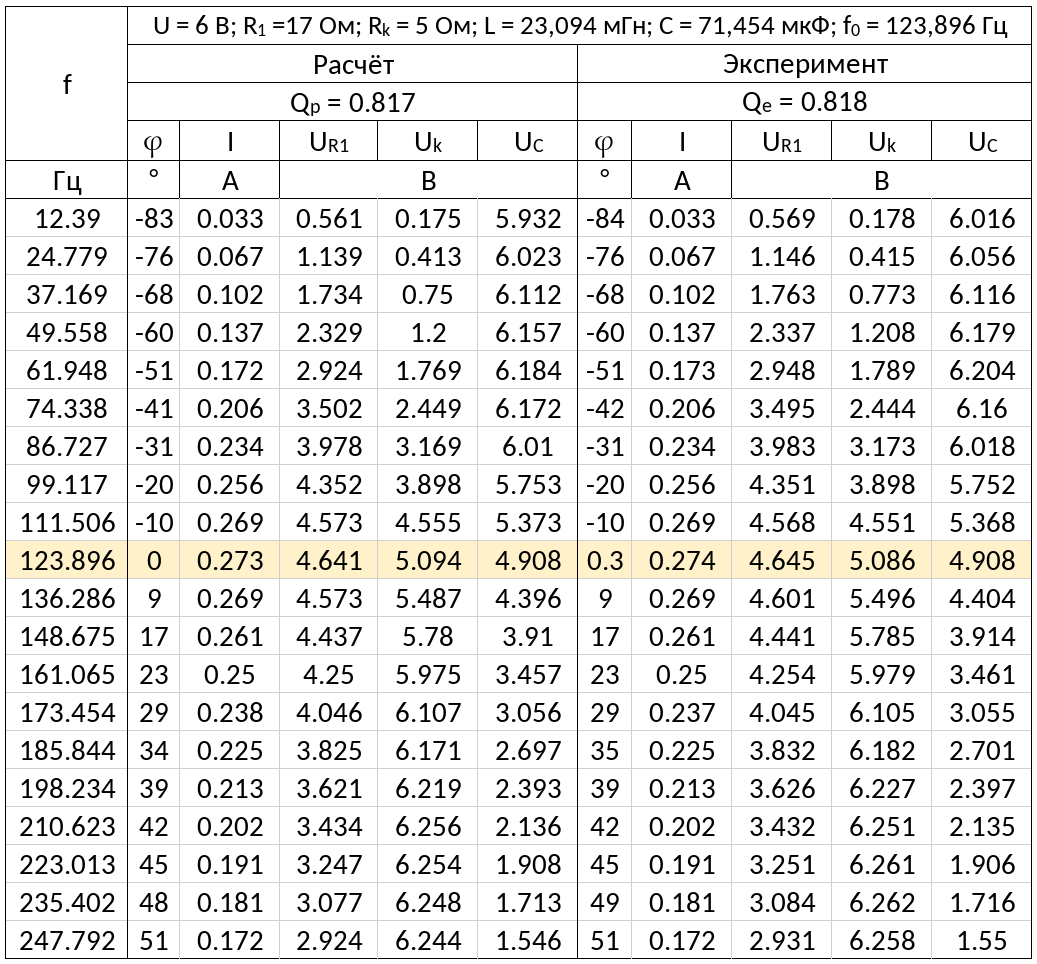
\includegraphics[width=1\textwidth]{./data/table_2-3.png}
	\caption{Итоговая таблица 2.3}
\end{table}
